\section{AI METHODS}  \normalfont

This section describes the approaches relevant to the work presented in this thesis. First, an introduction is given to the main area of the thesis,~\acrfull{ec}, followed by a brief introduction to~\acrshort{mape}. Finally,~\acrfull{ml} is briefly introduced and discussed.

%T, a First, a brief introduction is given into the main two areas: Evolutionary Computation (EC) and Machine Learning (ML).

% , to then continue into the specific approaches used. When applicable, it will be highlighted what was developed as part of the publications./

\subsection{Evolutionary Computation}

\acrfull{ec} is a subfield within~\acrshort{ai} inspired on Darwin's theory of evolution~\cite{darwin_origin_1859} and Darwinian principles of natural selection and evolution of population over generations to primary solve/optimize a problem or task, with the premise of ``survival of the fittest''.~\acrshort{ec} is a family of population-based algorithms that focuses on searching a multidimensional space for solutions through executing an iterative refinement loop. The basic premise is that by having a set of individuals in an environment to be experienced or with tasks to be solved, arises competition that causes natural selection, which results in finding high-performing solutions.~\acrfull{ea} is a subset of~\acrshort{ec}, which applies a set of evolutionary mechanisms in the refinement cycle: \textit{selection}, \textit{variation operators}, \textit{evaluation}, and \textit{replacement}~\cite{eiben_introduction_2007}.

A typical~\acrshort{ea} starts by \emph{creating} a set of random solutions in a multidimensional space and \emph{evaluates} them using some fitness function. Based on this measurement, solutions can be sorted, and better candidates can be \emph{selected} to seed the next generation and~\emph{variation operators} such as recombination or mutation can be applied to them to create a new set of candidates, i.e., the offspring. These solutions are once again~\emph{evaluated}, and compete against the current population to \emph{replace} it and become part of the next generation. This process is repeated until a solution of sufficient quality is found, which ends the execution. In such a loop, Eiben and Smith highlight two evolutionary mechanisms as fundamental for continuously producing and encountering high-performing individuals and creating diversity. The~\emph{selection} mechanism, which increases the pressure on selecting high-performing individuals for variation that ultimately results in increasing the quality of the population. The~\emph{variation operator}, which varies individuals to produce candidate solutions, creating the necessary diversity, and achieving novelty~\cite{eiben_introduction_2007}. 

% Pseudocode of the~\acrshort{ea} loop is shown in listing~\ref{alg:EA}

Moreover, under the subset of~\acrshort{ea} there exist four main variants:~\emph{Genetic Algorithms},~\emph{Genetic Programming},~\emph{Evolution Strategies}, and~\emph{Evolutionary Programming}. However, their distinction is mainly on the individuals' encoding, i.e., how each individual or solution is internally represented, which also limits what variant operators can be applied. For instance, Genetic Algorithms use genes encoded as finite strings, while Evolution Strategies' individuals are represented as real-valued vectors where approaches such as Covariance Matrix Adaptation could be applied~\cite{fontaine_covariance_2019}. Genetic algorithms are used for the work presented in this thesis. The content to be evolved (i.e., levels in a dungeon) is represented as a finite set of integers, and operators such as mutation and recombination through crossover can be applied.

\begin{figure}
    \centering
     \subfloat[Genotype\label{subfig-1:directGen}]{%
       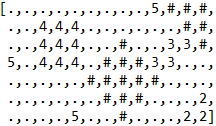
\includegraphics[width=0.45\textwidth]{figures/EC/directEncoding-gen2.png}
     }
     \hfill
     \subfloat[Phenotype\label{subfig-2:directPhen}]{%
       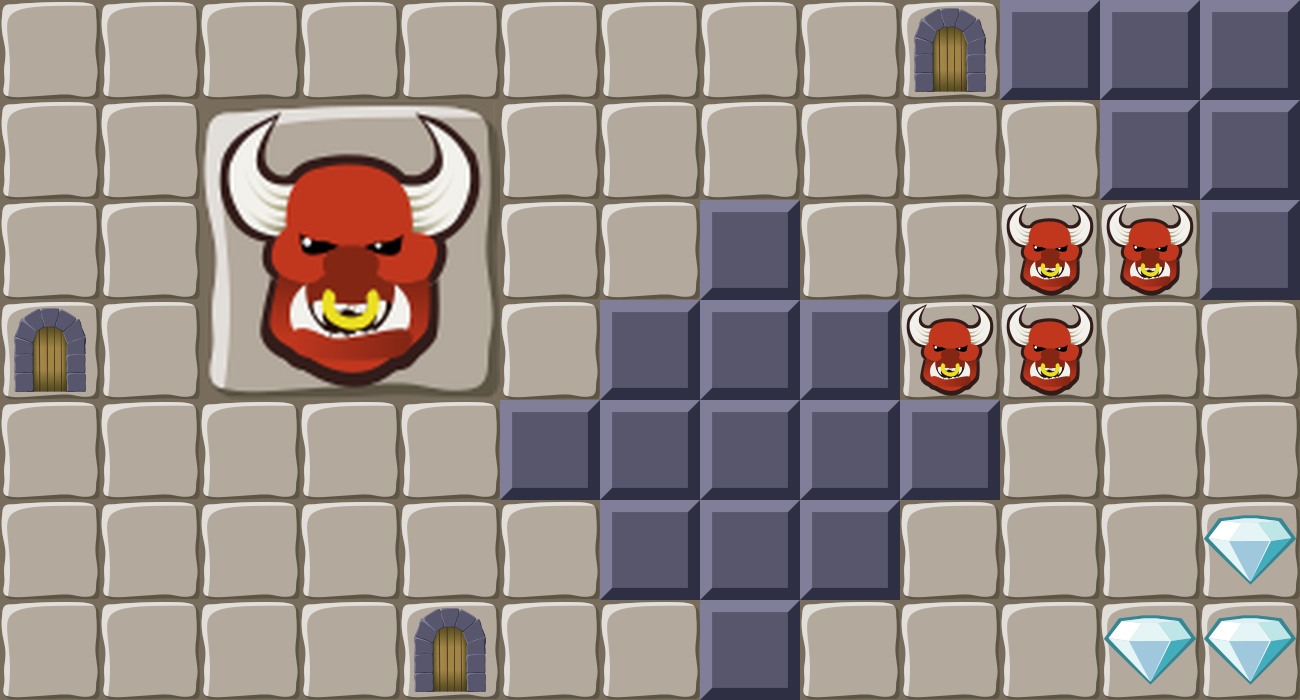
\includegraphics[width=0.45\textwidth]{figures/EC/directEncoding-phen.png}
     }
    
    \caption{Example of direct encoding}
    \label{fig:directENCOD}
\end{figure}

\subsubsection{Evolutionary Algorithm Components}

\paragraph{Representation}
Individuals (i.e., solutions) within a population have two representations: genotypes and phenotypes. \emph{Genotype} is the individual's internal representation within the~\acrshort{ea}, while \emph{Phenotype} is the ``translation'' of the genotype when acting in the environment. For instance, human genotypical representation is the DNA (genotype), while the body, brain, organs, etc. are the phenotypical representation. Such representation and translation are also called \emph{encoding}, which can fluctuate from direct to indirect encoding. 

Direct encoding refers that the genotype is mapped bit-by-bit to the phenotype. In contrast, indirect encoding refers to the opposite, the genotype is minimally encoded, and its representation does not match the phenotype. For instance, in the case of evolving tile-based rooms in a dungeon, a direct encoding could mean that the genotype is an array with integers, each denoting a space in the room and the corresponding tile in the phenotype (shown in figure~\ref{fig:directENCOD}). A lesser direct encoding could have the genotype be an array that groups together areas of the room and marks them as specific areas, or an even lesser let it just be a ruleset (such as in L-systems~\cite{prusinkiewicz_algorithmic_1996,shaker_evolving_2012}) to create the levels. Encoding and representation of individuals are one of the main challenges in~\acrshort{ea} since the encoding can drastically change the evolutionary mechanisms and how the content is generated and explored~\cite{ashlock_representations_2016,clune_performance_2011,stanley_compositional_2007}.

\paragraph{Evaluation}

In an~\acrshort{ea}, it is usually used a fitness function to assess the population and solutions. This estimates the quality of the solutions by testing some metrics that estimate and rank these solutions. Fitness functions are usually context-dependent and help solve the tasks at hand by using some representative heuristic of the task. For instance, if evolving levels in a game, quality can be measured based on the tile distribution or the challenge vs. reward. However, objective-based functions might not be the best way of evaluating content. Environments and tasks could be deceptive with a space filled with local optima, limiting the search; or diversity among the solutions might want to be rewarded rather than just ranking. Stanley and Lehman discuss such challenges with objective-based functions and proposed using divergent searches for stepping stones to solutions, with the aim of open-endedness~\cite{stanley_why_2015}. More work and discussion on this is presented in section~\ref{sec:Backqd}.

\paragraph{Selection}

Selection is used to choose the parents of the next generation of candidate solutions; thus, it chooses which individuals variation operators will be applied to. Selection approaches are biased towards selecting high-quality individuals; after all, these are the ones with the best chances to generate better candidates. However, to counter greedy strategies and avoid getting stuck in local optima, lower-quality individuals still get a chance to be selected (with a similar idea to tabu-search). 
% There are three main approaches to selection: \emph{roulette}: , \emph{tournament}: , and \emph{ranking}:.

\paragraph{Variation Operators}

Once individuals from a population are selected, a set of variation operators are applied to create candidates for the next generation. The operators might be \emph{Mutation} or \emph{recombination} as crossover. Mutation is applied to a single individual with the aims of varying some genes from the genotype to create variation and diversity. For instance, if mutation is not applied, the~\acrshort{ea} is limited to the genes encountered in the initial population; if a key gene was not produced, the global optima might never be found. Common mutation operators are to swap a gene for another in the genotype or randomly change a gene for a random value. Crossover requires at least two individuals that can, as the name indicates, cross their genes to form new candidates. Such is exemplified in figure~\ref{fig:crossoverEX}. The result of applying these operators to the selected parents is a set of candidate solutions (offspring) that are evaluated and compete against the current population for a place in the next generation.

\begin{figure}
\centerline{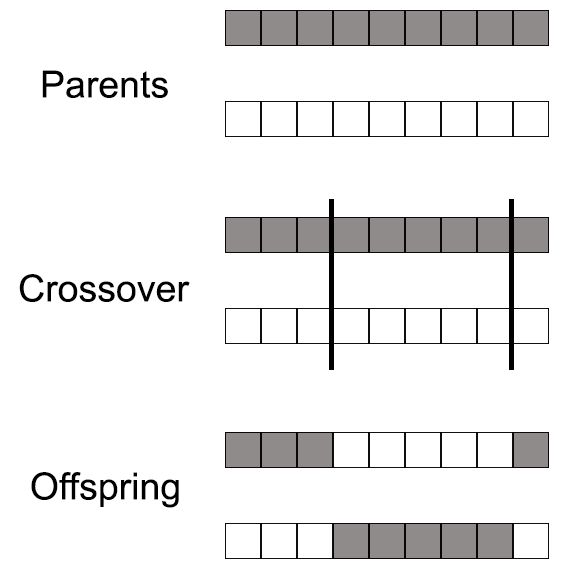
\includegraphics[width=0.5\textwidth]{figures/EC/crossover-example-bw.png}}
\caption{Example of the crossover variation operator
} \label{fig:crossoverEX}
\end{figure}

\paragraph{Replacement}

Replacement strategies mainly focus on replacing lower-quality individuals from the population for better candidates generated through the variation operators, hence, ``survival of the fittest''. However, as it will be explained in section~\ref{sec:map-elites}, not all~\acrshort{ea} work the same. Some have local competition with individuals with similar behavioral novelty~\cite{lehman_evolving_2011}; other approaches have competition among phenotypical similars to preserve innovations encountered in the search space~\cite{stanley_evolving_2002}.

% \begin{algorithm}
% \caption{Evolutionary Algorithm Loop}\label{alg:EA}
% \begin{algorithmic}
% \Procedure{EA}{}
% \State $POPULATION \gets RND\_SOLUTIONS$
% \State $EVALUATE$ each solution \textit{in} $POPULATION$
% % \State $a\gets b$
% % \Procedure{Euclid}{$a,b$}\Comment{The g.c.d. of a and b}
%   \State $r\gets a\bmod b$
%   \While{$r\not=0$}\Comment{We have the answer if r is 0}
%       \State $a\gets b$
%       \State $b\gets r$
%       \State $r\gets a\bmod b$
%   \EndWhile\label{euclidendwhile}
%   \State \textbf{return} $b$\Comment{The gcd is b}
% \EndProcedure
% \end{algorithmic}
% \end{algorithm}

% \subsubsection{Feasible-Infeasible two-Population}

% \begin{itemize}
%     \item What is FI-2Pop
% \end{itemize}

% \subsubsection{Interactive Evolution}

% \begin{itemize}
%     \item simple not extensive text about IE \cite{Takagi2001-InteractiveEvo}
% \end{itemize}

\subsubsection{MAP-Elites} \label{sec:map-elites}

\acrlong{qd} algorithms are a relatively new family of algorithms that leverage the strengths of divergence and convergence search~\cite{pugh_quality_2016}. One algorithm from this family is~\acrshort{mape}, which explores the space yielding a collection of high-performing and diverse solutions. The main characteristics of~\acrshort{mape} are: 1) that it returns a collection of high-performing yet diverse solutions to address multiple wanted behavioral characteristics, for instance, robots that can move around and have a set of different behaviors and characteristics~\cite{cully_robots_2015}. 2) Using behavioral features as dimensions and discretizing the space with cells helps the algorithm illuminate the search space and control niches of solutions. And 3) By using these features and cells, the algorithm is able to substantially explore the space finding in the way a greater amount of solutions than in other approaches.~\acrshort{mape} has been extensively evaluated and resulted in a far superior approach to convergence search (i.e., objective-based) or divergence search (e.g., novelty search) alone, and other~\acrshort{qd} approaches such as~\acrshort{nslc}~\cite{mouret_illuminating_2015}. 

\acrshort{mape}, while superior to other approaches, its iterative cycle is not that different as the one presented earlier in this chapter. The main changes that~\acrshort{mape} introduce are: 1) instead of having one population, the~\acrshort{ea} uses cells; and 2) besides the fitness function to calculate the quality of individuals, it requires a set of behavioral feature dimensions to divide the space into cells and where individuals will be stored. In the vanilla version of~\acrshort{mape}, each cell contains one individual, and as the search encounters new individuals within the same cell, the individual with higher-quality is kept, and the other is disregarded. This way, the algorithm is able to preserve only high-quality solutions while retaining diverse solutions. 

Moreover, the algorithm is shown in Listing~\ref{alg:mape}, which first initializes a collection of individuals evaluated with the fitness function and tested for their behavioral features to be placed in specific cells. Then random selection\footnote{Gravina et al. have experimented on using other selection approaches with beneficial and exciting results~\cite{gravina_blending_2019}} occurs on top of cells to pick individuals that then compete in a classical selection strategy (e.g., comparing fitness) to produce candidate solutions. Variation operators are applied to the selected parents, and the offspring are evaluated with the fitness function and tested for their behavioral features. Depending on the cell the offspring belong, they will need to compete if occupied with the current occupant or if unoccupied, the offspring is placed in the cell, and the cycle restarts. With such a simple algorithm,~\acrshort{mape} can encounter and return a collection of diverse and high-performing individuals. Firstly, this is due to the pressure in cells for high-performing individuals. Secondly, due to retaining individuals in these multidimensional cells, where they might be entirely different for another solution (e.g., have a complete different genotype) yet be as high-performing.


\begin{algorithm}
\begin{algorithmic}
\Procedure{MAP-Elites Algorithm (simple, default version)}{}
\State $(\mathcal{P} \leftarrow \emptyset, \mathcal{X} \leftarrow \emptyset)$
\For{iter $  = 1\to I$}
\If{iter $< G$} 
  \State $\mathbf{x'}\leftarrow $ random\_solution()  
\Else 
  \State $\mathbf{x}\leftarrow $ random\_selection($\mathcal{X}$) 
  \State $\mathbf{x'}\leftarrow $ random\_variation($\mathbf{x}$) 
\EndIf
\State $\mathbf{b'}\leftarrow $feature\_descriptor($\mathbf{x'}$) 
\State $p'\leftarrow $performance($\mathbf{x'}$) 
\If{$\mathcal{P}(\mathbf{b'})= \emptyset$ or $\mathcal{P}(\mathbf{b'})<p'$}
\State $\mathcal{P}(\mathbf{b'})\leftarrow p'$ 
\State $\mathcal{X}(\mathbf{b'})\leftarrow \mathbf{x'}$ 
\EndIf
\EndFor
\State \Return feature-performance map ($\mathcal{P}$ and $\mathcal{X}$)
\EndProcedure
\end{algorithmic}
\caption{Pseudocode description of the MAP-Elites Algorithm. Taken from~\cite{mouret_illuminating_2015}}
\label{alg:mape}
\end{algorithm}

%%UNCOMMENT FOR ADDING THE COMMENTS

% \begin{algorithm}
% \begin{algorithmic}
% \Procedure{MAP-Elites Algorithm (simple, default version)}{}
% \State $(\mathcal{P} \leftarrow \emptyset, \mathcal{X} \leftarrow \emptyset)$\Comment{\emph{Create an empty, $N$-dimensional map of elites:  \{solutions $\mathcal{X}$ and their performances $\mathcal{P}$\} }}
% \For{iter $  = 1\to I$} \Comment{\emph{Repeat for $I$ iterations.}}
% \If{iter $< G$} \Comment{\emph{Initialize by generating $G$ random solutions}}
%   \State $\mathbf{x'}\leftarrow $ random\_solution()  
% \Else \Comment{\emph{All subsequent solutions are generated from elites in the map}}
%   \State $\mathbf{x}\leftarrow $ random\_selection($\mathcal{X}$) \Comment{\emph{Randomly select an elite $x$ from the map $\mathcal{X}$}}
%   \State $\mathbf{x'}\leftarrow $ random\_variation($\mathbf{x}$) \Comment{\emph{Create $x'$, a randomly modified copy of $x$ (via mutation and/or crossover)} }
% \EndIf
% \State $\mathbf{b'}\leftarrow $feature\_descriptor($\mathbf{x'}$) \Comment{\emph{Simulate the candidate solution $x'$ and record its feature descriptor $\mathbf{b'}$}}
% \State $p'\leftarrow $performance($\mathbf{x'}$) \Comment{\emph{Record the performance $p'$ of $x'$}}
% \If{$\mathcal{P}(\mathbf{b'})= \emptyset$ or $\mathcal{P}(\mathbf{b'})<p'$}\Comment{\emph{If the appropriate cell is empty or its occupants's performance is $\leq p'$, then}}
% \State $\mathcal{P}(\mathbf{b'})\leftarrow p'$ \Comment{\emph{store the performance of $x'$ in the map of elites according to its feature descriptor $\mathbf{b'}$}}
% \State $\mathcal{X}(\mathbf{b'})\leftarrow \mathbf{x'}$ \Comment{\emph{store the solution $x'$ in the map of elites according to its feature descriptor $\mathbf{b'}$}}
% \EndIf
% \EndFor
% \State \Return feature-performance map ($\mathcal{P}$ and $\mathcal{X}$)
% \EndProcedure
% \end{algorithmic}
% \caption{Pseudocode description of the MAP-Elites Algorithm. Taken from~\cite{Mouret2015}.}
% \label{alg:mape}
% \end{algorithm}

Furthermore,~\acrshort{mape} have become popular and attractive due to all the abovementioned benefits and characteristics, which have not only spread it's use in many fields and many experiments but also sparked many variations. The Constrained~\acrshort{mape} by Khalifa et al.~\cite{khalifa_talakat_2018} is the one this thesis relies on and has expanded. Their approach added populations in each cell rather than individuals, preserving even more solutions, and combined~\acrshort{mape} with~\acrshort{fi2pop}, which yielded two populations per cell, one driven by the fitness and the other driven by satisfying a set of constraints. Through this, they applied the same process as with the vanilla~\acrshort{mape} but per population (i.e., feasible and infeasible), which resulted in useful and interesting results for the generation of bullet hells bosses.

%%%%%%%%% HERE IS WHERE ICMAPE WAS

% Our fitness function being adaptable

%  this would only focus on obtaining one high-performing individual, 2) the search would focus in fewer places of the generative space, and as a consequence, 3) the diversity of the generated individuals would be scarce. T

% explores the behavioral space for a collection of solutions that are both high-performing and diverse among each other, with the caveat that~\acrshort{mape} discretizes the behavior space as a grid of cells informed by a set of feature dimensions that illuminate the behavior space.

\subsection{Machine Learning}

\acrfull{ml} is a sub-field of~\acrshort{ai} that focuses on using learning algorithms that can learn from data and that are trained through some strategy such as supervised learning or reinforcement learning~\cite{goodfellow_deep_2016}. Formally (and generally), learning in~\acrshort{ml} was operationally defined by Mitchell~\cite{mitchell_machine_1997} as: “A computer program is said to learn from experience \textit{E} with respect to some class of tasks \textit{T} and performance measure \textit{P}, if its performance at tasks in \textit{T}, as measured by P, improves with experience \textit{E}.” 

The task~\textit{T} in~\acrshort{ml} is not the learning \textit{per se}, rather learning is the way to attain the ability to solve the tasks.~\acrshort{ml} helps us solve complex tasks that are deemed too complex to be solver by fixed programs such as the creation of games~\cite{summerville_procedural_2018} or playing games~\cite{mnih_human-level_2015,justesen_deep_2020}. Tasks in~\acrshort{ml} might be a \emph{classification} task: what category \textit{k} an input belongs~\cite{clanuwat_kuronet_2019}; a \emph{regression} task: where it is asked to predict some numerical value based on some input; \emph{synthesis} task: create new examples based on the training samples~\cite{torrado_bootstrapping_2020}; or \emph{machine translation} task: translate an input from one language to another~\cite{hartmann_comparing_2019}.

Moreover, performance~\textit{P} relates to how a learning model is assessed to check that it is learning from experience~\textit{E} to tackle task~\textit{T}. Depending on the type of task that the model must solve, the performance measure would vary, as it is dependant on it, similarly as to how fitness functions are dependant on the problem to be solved. The usual performance measures used are \textbf{accuracy} and \textbf{error rate}. For tasks such as image generation the \textbf{inception score} is normally used~\cite{salimans_improved_2016} or for machine translation the \textbf{BLEU} is used to measure the quality of the translated text~\cite{papineni_bleu_2002}. The key aspect when evaluating performance in a task is that the learning model should be tested with data it has not used for learning, thus showing the ability of the model to solve "unknown" tasks~\cite{goodfellow_deep_2016}. 

Furthermore, experience~\textit{E} is related to the data and examples provided to the tool and what strategy is used to train a learning model. Learning strategies in~\acrshort{ml} can be categorized in two main learning strategies: \emph{Supervised} and \emph{Unsupervised} learning. However,~\acrfull{rl} has gained tremendous interest from the research community, and is the current learning strategy that is used to solve many tasks due to the metaphor regarding how human's learn and the fact that the learning happens by experiencing the environment rather than learning the data~\cite{juliani_obstacle_2019}.~\acrfull{ssl} has also been gaining popularity as an approach to move away from traditional supervised training by not using human-annotated dataset to learn representations of data~\cite{doersch_multi-task_2017}.

Within~\acrlong{pcg} and games,~\acrshort{ml} has been increasingly used, gaining popularity to generate different types of content.~\acrshort{pcg} via~\acrshort{ml} is a prospect area that encompasses all algorithms and approaches where the generated content is the output of models trained on existing content~\cite{summerville_procedural_2018}. On the other hand,~\acrshort{ml} can take advantage of~\acrshort{pcg} approaches that continuously create content to increase generality, as discussed by Risi and Togelius~\cite{risi_increasing_2020}. Moreover, Liu et al. discuss the different deep learning approaches used thus far for~\acrshort{pcg}, the open areas for research, and more in detail on the benefit of these approaches both for the deep learning community and the~\acrshort{pcg} community~\cite{liu_deep_2020}.

%or instance, they have the opportunity to be used to increase the generality of~\acrfull{ml} approaches~\cite{Risi2020-pcgGeneralityML},

%%Discuss 
% Over the past years,~\acrshort{ml} has gain popularity in the field of~\acrshort{pcg} in what is called~\acrshort{pcg} via~\acrshort{ml}~\cite{summerville2018procedural}. 
% ~\acrshort{pcg} via~\acrshort{ml} is a prospect area that have shown exciting results for generating a vast amount of game content. Yet creating game levels~\cite{Snodgrass17-GenerateMapsMArkovModels}  for approaches 
% Approaches using supervised learnin
% With datasets such as the Video Game Level Corpus~\cite{Summerville2016-vglc}, many approaches have been 


%%%%%%%%% HERE IS WHERE DESIGNER PREFERENCE AND DESIGNER PERSONAS WAS
%%%%%%% I think perhaps i need to then write about active learning and those things, and sequential mining and clustering approaches.

